\section{Methodology}
\label{ch: methodolgy}

% \textbf{todo: keuze bolling ipv holling toelichten}
The objective of this thesis is to increase the feasibility of a floating island by using a structure that attenuates the wave energy. The procedure to achieve this objective is to optimise the design of such a structure with the \acrfull{cfd} program ComFLOW and the design method: \acrfull{doe}. In this section, a methodology is discussed on how this optimisation is going to be realised. \\
\\
The literature review resulted in a scope and some decisions. A fundamental choice about the setup of the breakwater was made quite early in the process, which is discussed in Section \ref{sec: choice setup}. ComFLOW has never been used before to quantify the performance of floating breakwaters. Therefore, the validation in this application seemed crucial. The methodology of this part of the project is reported in Section \ref{sec: methodology validation}. The remaining part of the project consists of the actual optimisation of the breakwater, from which its methodology is described in Section \ref{sec: methodology design optimisation}. \\



\section{Choice in setup: connected to or floating in front the island}
\label{sec: choice setup}
% Floating  breakwaters  are  held  in  place  by  mooring  lines  or  piles,  with  piled  mooring  being  suitable  only at shallow sites (McCartney, 1985).  The mooring lay-out requires careful design to environmental conditions,not only from a structural and mooring integrity point of view, but also because the mooring stiffness affects the attenuation performance of the breakwater (Loukogeorgaki et al., 2017).  A stiffer mooring system tends to lead to better wave attenuation performance (Loukogeorgaki and Angelides, 2005).  Consistently, a captives etup (all degrees of motions restrained) or piled setup (structure can only move vertically) generally induce stronger  wave  attenuation  than  a  moored  setup  (Ruol  et  al.,  2012).   An  exception  is  the  attenuation  at  the wave frequencies corresponding to one of the natural frequencies of the moored floater,  which can be higher for a moored compared to captive setup because of enhanced viscous dissipation induced by resonant motion behaviour  (Ruol  et  al.,  2012;  Ji  et  al.,  2018).   At  the  same  time,  resonant  motion  behaviour  leads  to  high instantaneous mooring loads (Loukogeorgaki and Angelides, 2005) and it is therefore recommended to design the mooring system based on second-order rather than first-order wave excitation (Drimer et al., 1992)


The floating breakwater could be placed a certain distance in front of the floating island (a so-called stand-alone setup), while it is moored by itself and interacts with the waves way before they arrive at the floating island. Or it could be connected to the floating island itself, where it catches the waves just before they can interact with the structure. Both setups have their pros and cons; a stand-alone setup is easier to move and, therefore, widely applicable. But when this breakwater is connected to a floating island, a better wave attenuation performance is expected.\\
\\
Numerical and experimental studies showed that the stiffness of the mooring system of the floating breakwater affects the attenuation of the waves. A stiffer mooring system has a better wave attenuation performance \citep{Loukogeorgaki2006} \citep{Loukogeorgaki2017}. A floating breakwater with pile setup, where only a heave motion is allowed, showed better performance than softly moored \citep{Ruol2012}. Consequently, a fully captive set-up (where all degrees of freedom are restrained) is expected to give the most promising results. This resulted from the experimental study \citep{Zanden2021}, where a submerged parabolic beach that enforced wave energy dissipation through breaking, was tested both in a soft moored setup and a captive setup. As expected, the captive setup had significantly better wave attenuation performances. The motions of a floating island are naturally much less than those of a smaller stand-alone floating breakwater, so more stiffness can be imposed when the floating breakwater is connected to the structure. This is why the connected setup is expected to have better wave attenuation performances. 
Also, when looking at a stand-alone setup, higher waves will form again on the lee-side of the floating breakwater due to wave diffraction around the structure \citep{Holthuijsen2007} \citep{Zanden2021}. In other words, when using the stand-alone setup, which is placed further away from the floating island, the floating breakwater must be wider to achieve the same wave attenuation results. Thus, the choice has been made to make a design of the floating breakwater that is connected to the floating island. \\
\\


\section{Validation}
\label{sec: methodology validation}

The validation of this experiment is done to get used to the software and find the right settings and grid outline, which minimises the computational power required while giving stable simulations and reliable results.\\
\\
When a wave interacts with a breakwater, the wave energy is transmitted through, reflected back, or dissipated at the location of the breakwater. Each of these phenomena was found to be an important quantity to validate in order to judge whether the ComFLOW results are reliable. Wave transmission and forces on the structure will be recorded in ComFLOW simulations with a box-type breakwater, to make a comparison with the analytical formulas: the Macagno formula (equation \ref{eq: macagno1953}) and formula \ref{eq: longuethiggins force} derived by Longuet-Higgins. The Macagno formula predicts wave transmission, and formula \ref{eq: longuethiggins force} describes the forces on a box-type breakwater. Both these formulas are derived from linear wave theory.\\
\\
To track whether ComFLOW handles wave dissipation through wave breaking well and investigate what grid size should be used, a comparison will be made with an experiment in which waves were plunging over a breaker bar for different grid refinements in ComFLOW. The wave transmission after the moment of breaking will be recorded in ComFLOW and compared to the results of the experiment. 



\section{Design optimisation}
\label{sec: methodology design optimisation}
The design optimisation is explained in three different parts: the parametrisation of the breakwater geometry is discussed in \ref{subsec: methodology parametrisation}, the use of \acrfull{doe} in \ref{subsec: methodology doe} and how the simulations need to be handled in ComFLOW in \ref{subsec: methodology comflow}.

\subsection{Parametrisation of breakwater}
\label{subsec: methodology parametrisation}
A floating breakwater must attenuate the wave energy through dissipation and reflection. The literature review in Chapter \ref{ch:literaturereview} showed that a box-type breakwater is capable of reflecting much of the wave energy and an inclined beach under the water surface forces the waves to break and thus dissipate the wave energy. With that in mind, the breakwater is parameterized in such a way that it can take both these forms and many in between. 


\begin{figure}[h]
    \centering
    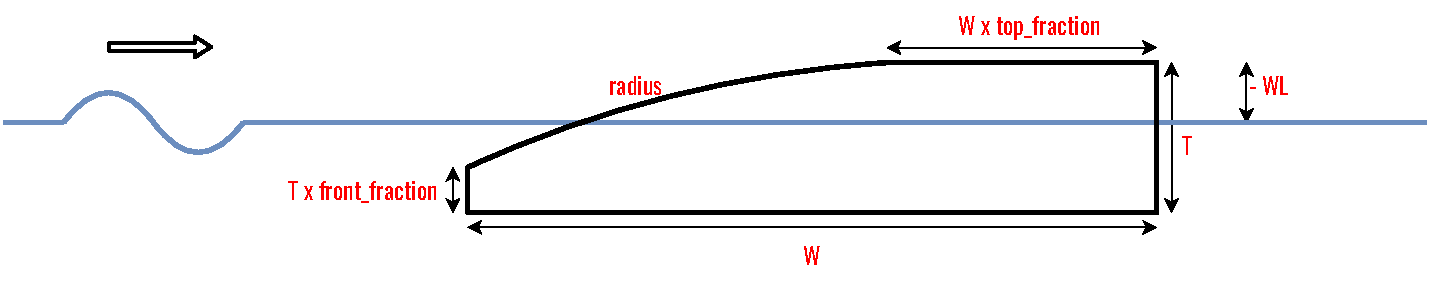
\includegraphics[width = \linewidth]{figures/Methodology/parametrisation.pdf}
    \caption{parametrisation of breakwater}
    \label{fig: parametrisation breakwater}
\end{figure}

The six different parameters (shown in Figure \ref{fig: parametrisation breakwater}) will have the following boundaries, and more elaboration is given below:
\begin{enumerate}
    \item W [m]: dimension in x-direction
    \item T [m]: dimension in z-direction
    \item top\_fraction (0,1): is a fraction of the variable W, such that the length of the top can not exceed the bottom 
    \item front\_fraction (0,1): is a fraction of variable the T, such that the length of the front can not exceed the aft 
    \item radius [m]: the curve of the inclined beach
    \item WL [m]: shift of the water level from the top of the breakwater. 
\end{enumerate}

Here, the fractions (parameters 3 and 4) are values between 0 and 1 so that the front side of the breakwater cannot exceed the depth \textit{T} and the top side cannot exceed the width \textit{W}. The beach is shaped by plotting part of a circle through the locations where the circle crosses the top and the front of the breakwater. The beach curve is varied by changing the radius of this circle (parameter 5). Parameter 6, which defines the z-position of the breakwater, changes the waterline with regard to the origin of the body-fixed coordinate system. For example, with WL = 1 the origin of the body-fixed coordinate system is one metre under the waterline and WL = -1 means that the body-fixed origin is one metre above the waterline.



\subsection{\acrfull{doe}}
\label{subsec: methodology doe}
As discussed extensively in Section \ref{sec: DoE}, \acrshort{doe} is used to make a \textit{design space}, which creates different configurations of the breakwaters, based on the parameters of interest. Then, after the performance of each configuration is quantified using the data from ComFLOW, the dependence of each parameter on the wave attenuation performance and the mean wave drift force can be traced. Then, a sequence of optimal breakwaters will be found ranked according to their desirability.



\subsection{ComFLOW simulations}
\label{subsec: methodology comflow}
ComFLOW will be used to quantify the performance of each configuration. It is investigated how each configuration performs by recording the transmitted wave height and the average surge force on the geometry. These quantities will be translated into a transmission coefficient and a mean wave drift force. 


\subsubsection{Waves}
The design optimisation is done with two different wave conditions, from now on referred to as \textbf{Wave Condition 1} and \textbf{Wave Condition 2}. For both, the characteristics are shown in Table \ref{tab: wave conditions}. Wave Condition 2 is the most extreme wave condition expected to occur in the North Sea in 100 years \citep{Fery2019}. This condition is important to test since the mean wave drift force of the floating island scales with the incoming wave height squared, and so the mooring system needs to be designed for this situation. Its group velocity is 9.69 m/s. Therefore, the first waves arrive at x = 580 m (this is an important position since this is the outer position where the wave height will be recorded; more about this in Section \ref{sec: post processing by Python}) at t = 60 seconds and approximately 23 wave periods will pass until the end of the simulation (t=300 s). To investigate how the optimal breakwater depends on the wave characteristics, the second wave condition is implemented. These waves will arrive at x = 580 m after 120 seconds, and from that moment exactly 30 waves are expected to pass. 

% Please add the following required packages to your document preamble:
% \usepackage{booktabs}
\begin{table}[h]
\begin{tabular}{@{}ccccccccc@{}}
\toprule
Wave Condition & Type    & H {[}m{]} & T {[}s{]} & $\lambda$ {[}m{]} & k {[}m$^{-1}${]} & kh {[}-{]} & c$_p$ {[}m/s{]} & c$_g$ {[}m/s{]} \\ \midrule
1              & Regular & 3.00      & 6.00      & 55.59            & 1.11E-1          & 2.60       & 9.26            & 4.90            \\
2              & Regular & 9.00      & 10.40     & 133.90           & 4.69E-2          & 1.08       & 12.88           & 9.69            \\
 \bottomrule
\end{tabular}
\caption{Two wave conditions used in design optimisation}
\label{tab: wave conditions}
\end{table}


In the simulations, some numerical dissipation causes the actual wave heights, which are interacting with the structure, to be a bit lower. For Wave Condition 2, the actual incident wave height is 2.67 metres, and for Wave Condition 2 it is 8.65 metres.



% \section{parametrisation breakwater}

% \section{Setup simulations}

% -comflow.cfi file with tags, with locations, mass, radius of intertia, attachment point, grid and everything else that is scripted\\
% -stijfheid fenders Table 2-4 van D10.4 S@S:
% \begin{itemize}
%     \item Axial Stiffness = 52.38 MN/m
%     \item Traverse Stiffness = 42.08 MN/m
%     \item Bending Stiffnes = 132.78 MNm/rad
% \end{itemize}
% On S@S project, the 45 m modules had two of these fenders at each side of an island module. So to compute these stiffnesses needed per unit width of breakwater, all the values are multiplied by two and divided by 45. This gives the stiffnesses used in the ComFLOW simulations:
% \begin{itemize}
%     \item Axial Stiffness = 2.33  MN/m
%     \item Traverse Stiffness = 1.87 MN/m
%     \item Bending Stiffnes = 5.90 MNm/rad  * 5 NOTE, FIVE TIMES THE FENDERS
% \end{itemize}

% -z-stijfheid vender:
% \begin{itemize}
%     \item aanname: hydrodynamische stijfheid één eilandmodule W=45, T = 6m
% \end{itemize}


% -check met box onder water of locatie fender goed zit!

% -z-stiffness too stiff. fender s@s/golfhoogte misschien juist (dan met maximale uitslag neemt hij kracht aan van fender stiffness bij 1 m exitatie).



\section{Scripting in Python}
Once a design space is created with the help of \acrshort{doe}, all the different configurations with its parameters are known. Then Python is used to prepare and start all simulations automatically. How this is done is explained in Section \ref{sec: preperation of simulations by Python}. Once the ComFLOW simulations are done, Python is also used to change the raw data into interpretable quantities. How these quantities are exactly calculated out of the raw ComFLOW output is explained in Section \ref{sec: post processing by Python}

\subsection{Preparation of simulations}
\label{sec: preperation of simulations by Python}
\subsubsection{Determining mass, radius of inertia and CoB of geometries}

The mass of each configuration is determined by the volume of the underwater body. To determine this, the body is divided into three areas, denoted by the green numbers in Figure \ref{fig: Figure for mass calculation}. The volume per unit width of area 1 is $W\cdot T\cdot front\_fraction$. The volume per unit width of area 2 is $|x_{WL}|\cdot W\cdot top\_fraction$. The volume per unit width of area 3 is computed numerically with the help of Python. The sloping beach is defined as two arrays, each containing a thousand characters, one defining the beach in z-direction and the other in x-direction. These arrays are used in a for-loop to do the calculation. With the three areas and the location of the waterline known, the total displacement per unit width of the breakwater ($\nabla_{breakwater}$) can be established. Then the mass of the breakwater is nothing less than multiplying that number with the density of the water which is used in ComFLOW: 1000 $kg/m^3$. 

% Symbolically this looks like
% \begin{equation}
%     m_{breakwater}  = \nabla_{breakwater} \cdot \rho_{water}
% \end{equation}
% per unit width of breakwater.\\
% \\

\begin{figure}[h]
    \centering
    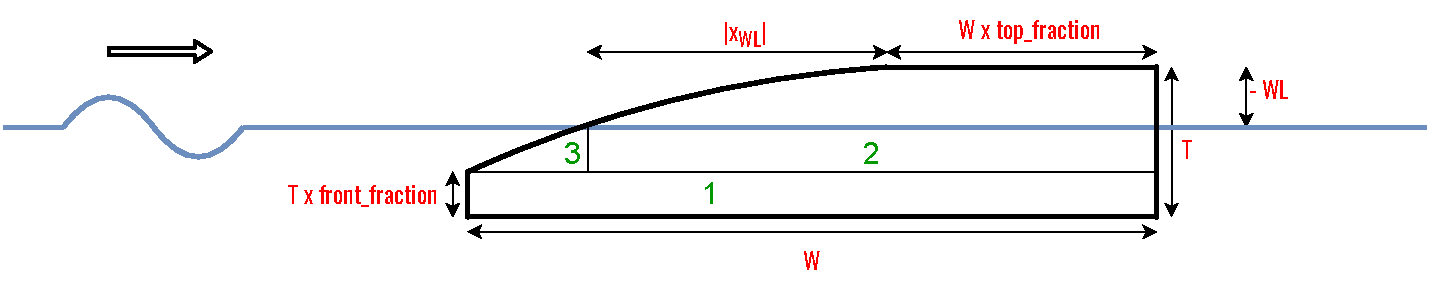
\includegraphics[width=\linewidth]{figures/Methodology/parametrisation_areas.pdf}
    \caption{Division of areas used in calculation of mass breakwater}
    \label{fig: Figure for mass calculation}
\end{figure}

In determining \acrfull{cob} of all geometries, the same division in areas is used. First, the focal point of each area is determined. Area 1 \& 2 both have a very straightforward focal point, and the one of area 3 is again done discretely using Python in the same for-loop as in the calculation of the mass of the breakwater. \\
\\
Since the simulations will be 2D, only pitch rotations occur, so the radius of pitch inertia ($k_{yy}$) must be calculated. For this, the assumption is made that the mass is uniformly distributed over the breakwater. Then the breakwater is divided into finite elements. Each element contributes to the radius of pitch inertia by
\begin{equation}
    k_{yy} = \sqrt{\frac{1}{12}(W^2 + H^2) + d^2}
\end{equation}
where $W$ is the width of that element, $H$ is the height and $d$ is the distance to the \acrfull{cog}. How this is scripted exactly can be seen in Appendix \ref{app: scripts for setting up simulations}.

\subsubsection{Stiffness hinge point with moving breakwaters}
Waves that interact with breakwaters create fluctuations in the pressure around the structure and create motions that the structures in reality have. Therefore, some breakwaters that come out of the optimisation will be resimulated in ComFLOW with an allowance of movement in pitch and surge direction, to map the influence of movements on the results of the optimisation. The presence of a floating island on the lee-side of the breakwater is imitated by defining a hinge point, on the lee-side of the breakwater on the water line (x=450m and z=0m). In 2D simulations, the breakwaters have three degrees of freedom: surge, heave, and pitch. The surge (translation in the x-direction) and the pitch (rotation around the y-axis) with respect to the hinge point will be allowed, and heave is restricted because most of the simulations showed strange unrealistic behaviour of the motions of the breakwaters and eventually caused the simulations to get unstable in most cases. \\
\\
The hinge point is defined in both the body-fixed coordinate system and the general (grid-fixed) coordinate system, and a spring term is imposed between these points. The fenders used for the design of the floating island of Space@Sea have an axial (surge) stiffness of 52.38 MN/m  per fender \citep{S@S_demonstationatwavetank}. Each 45 m wide module had two fenders, so the surge stiffness per unit width of the floating island is ($\frac{52.38 \cdot 45}{2}$) 2.33 MN/m. This value will be used for future simulations. The pitch stiffness of these fenders could not simply be used from the Space@Sea project, because this would cause some breakwaters to resonate in their pitch motion (i.e., their pitch stiffness around the hinge point would coincide with the hinge pitch stiffness). Therefore, the pitch stiffness imposed by the hinge point will be different for each breakwater: 1\% of its own hydrodynamic pitch stiffness with respect to the hinge point. Since there is no restoring moment for completely submerged breakwaters, 1\% of the restoring force of similar breakwater crossing the waterline, with a depth of two meters, is used for the submerged bodies. 




\subsection{Post-processing}
\label{sec: post processing by Python}
ComFLOW gives a raw output that needs to be modified into quantitative parameters to interpret them as perceptible parameters. This section discusses how this is done for the wave transmission of the breakwater and the drift forces on the geometries.



\subsubsection{Mean Wave Drift force}
At each timestamp in ComFLOW, the pressure is determined in each cell, with unit $N/m^2$. To arrive at the force acting on a geometry, the pressure of the cells around the body is integrated. Integrating the pressure in the yz-plane results in a net surge force $F_x$, integrating in the xy-plane in a heave force $F_z$ and for 3D simulations the sway force $F_y$ can be determined by integrating the pressure points in the zy-plane. Since the simulations in this thesis are in two dimensions (x and z), the y-dimension does not exist. Therefore, to obtain the force $F_x$, the pressure left and right of the geometry is integrated in only the dimension z and, therefore, the net resulting force will be a force per unit width of the breakwater, with unit $N/m$.\\
\\
With this in mind, it is understandable that a minimum amount of cells in the z-direction of the body is required to give applicable results for the surge force $F_x$. What this minimum is, is investigated in the validation phase of this thesis and resulted in 20 cells. The smallest dimensions of the cells of the grid around the breakwater are 125 mm. With smaller cells, the time step will be too small, which results in long execution times. Therefore, the minimum depth of the breakwater is 2.5 m. Then, the minimum number of cells along the z-direction of the geometry is 20. When the depth is greater than 5m, cell dimensions of 250mm are used to save execution time. \\
\\
The raw force output of ComFLOW is subject to high-frequency oscillations as a result of high-frequency local fluid pressures acting on the body. Therefore, this signal is filtered (purple line in Figure \ref{fig: methodology Fd calculation}). Also, the run-up (the time it takes for the waves to develop fully throughout the complete domain) is cut off. The simulation time is shortened so that an integer number of oscillations is taken into account (orange line). Then, the mean of the raw output (blue line) within this determined simulation time is taken to determine a single value for the mean wave drift force for each configuration of breakwater (green line). How this is done exactly can be observed in the function \textit{mean\_wave\_drift\_force} in Python script \ref{script: post processing functions} in Appendix \ref{app: scripts for post-processing}. The calculations of the \acrshort{cog} and radius of inertia were verified by comparing the results with analytical formulations for different box-type structures, producing the same results.\
In the results addressed in Chapter \ref{ch: captive design optimisation}, the mean wave drift force is non-dimensionalised by dividing it through the mean wave load on a wall with the same wave characteristics. From now on, this quantity will be called F$_{d,norm}$. As in the following equation:
\begin{equation}
    F_{d,norm} = \frac{\bar{F_d}}{\frac{1}{8}\rho g H_i^2}
    \label{eq: handling Fdnorm}
\end{equation}



\begin{figure}[H]
     \centering
     \begin{subfigure}[b]{0.49\textwidth}
         \centering
         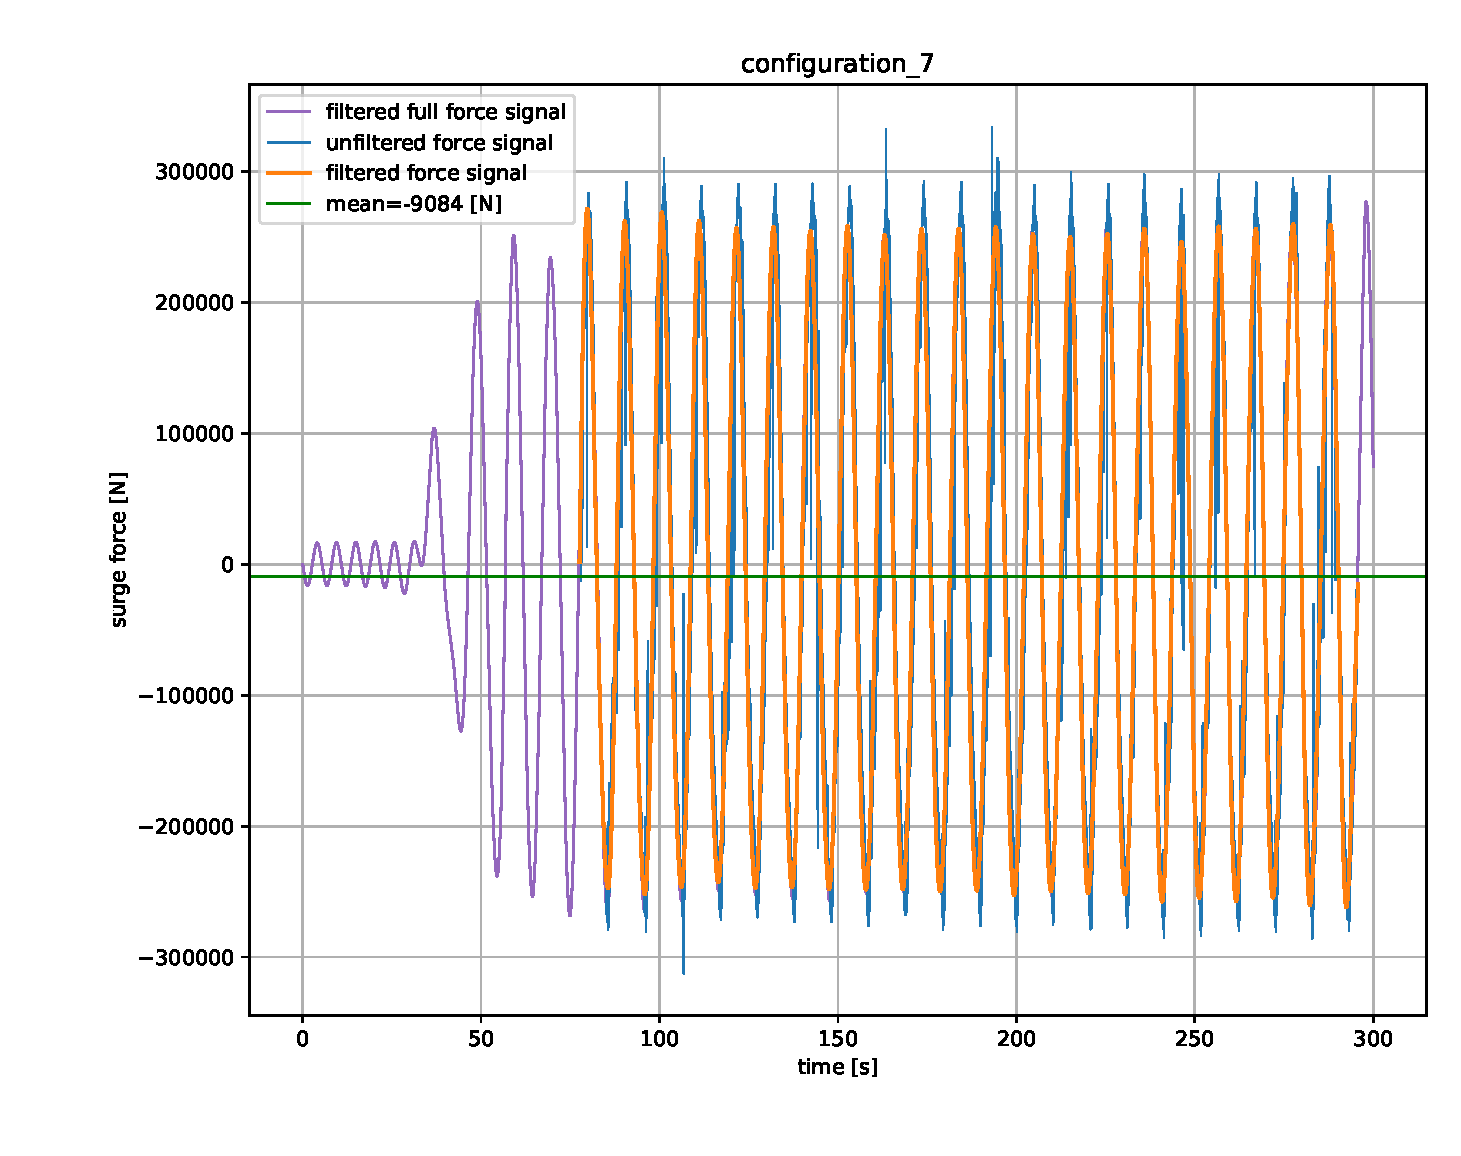
\includegraphics[width=\textwidth]{figures/Methodology/calculation_Fd_mean_methodology.pdf}
        \caption{Force signal used in calculation mean wave drift force}
        \label{fig: methodology Fd calculation}
     \end{subfigure}
     \hfill
     \begin{subfigure}[b]{0.49\textwidth}
         \centering
        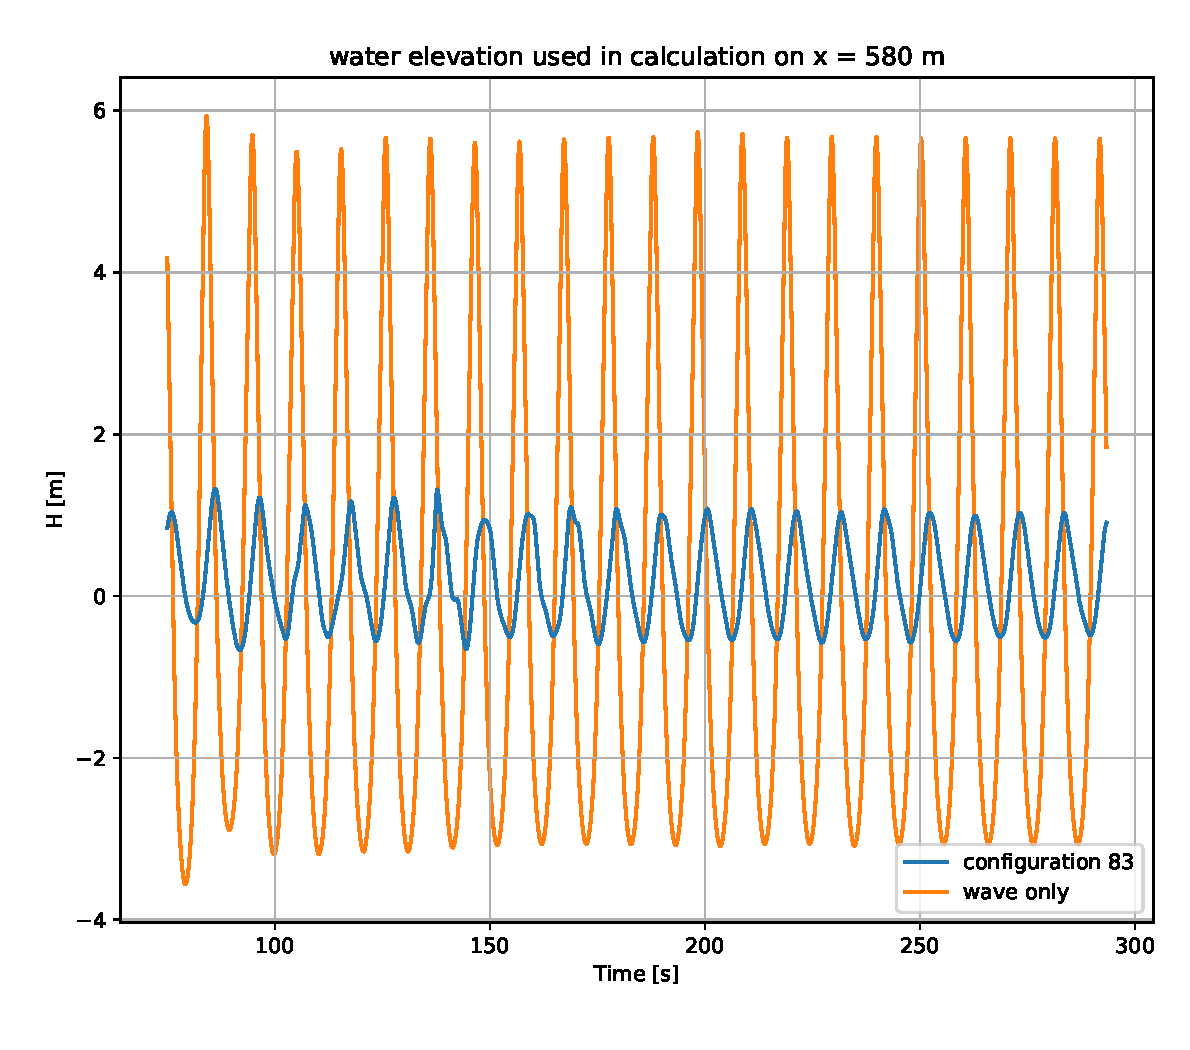
\includegraphics[width = \linewidth]{figures/Methodology/calculation_H_t_methodology.pdf}
        \caption{Wave elevation over time use in calculation wave transmission}
        \label{fig: methodology Kt calculation}
     \end{subfigure}
     \caption{Signals used in post-processing}
\end{figure}

\subsubsection{Wave transmission}
To understand how wave transmission is determined from ComFLOW output, it is necessary to understand how the grid is built, which will be used in the simulations (see Figure \ref{fig: grid used methodology}). The outline of this grid is determined in the validation phase of this thesis, which is extensively discussed in Section \ref{sec: general outline grid}. Here, the waterline is at z = 0, and the waves will be generated at the left boundary (x = 0) and propagate to the right. They will interact with the breakwater, which is placed up to x = 405 m. Therefore, the x-location of the left side (wave-ward) side of the structure depends on its width and its right side (lee-ward) is always placed at x=405m. Figure \ref{fig: zoomed grid used methodology} shows the grid more closely zoomed in on the position where the breakwater is placed. \\
\\
The transmitted wave height $H_t$ will be determined between x = 450 m and x = 580 m. At every cell at the waterline, the wave height over time is logged and can be read in Python. An example of the elevation of the water over time for a single cell (located at x=580m in the domain) of an arbitrarily chosen simulation (excluding run-up) is shown in Figure \ref{fig: methodology Kt calculation}. The average transmitted wave height is determined for every cell between x=450m and x=580m. Averaging this number leads to the value of the transmitted wave height $H_t$. Also, a 'wave-only' simulation is done, where the exact same settings are used, but without any geometry. The average wave height over time between x = 450 m and x = 580 m of this wave-only simulation is what is used as the incident wave height $H_i$ in the calculation of each of the transmission coefficients of the breakwater $K_t~=(H_t/H_i)$. This is done to account for the numerical dissipation that occurs between x = 0m and x = 580m. For this, the function \textit{transmitted\_wave\_height} in the Python script shown in Section \ref{script: post processing functions} of Appendix \ref{app: scripts for post-processing} is used. \\
\\

\begin{figure}[h]
    \centering
    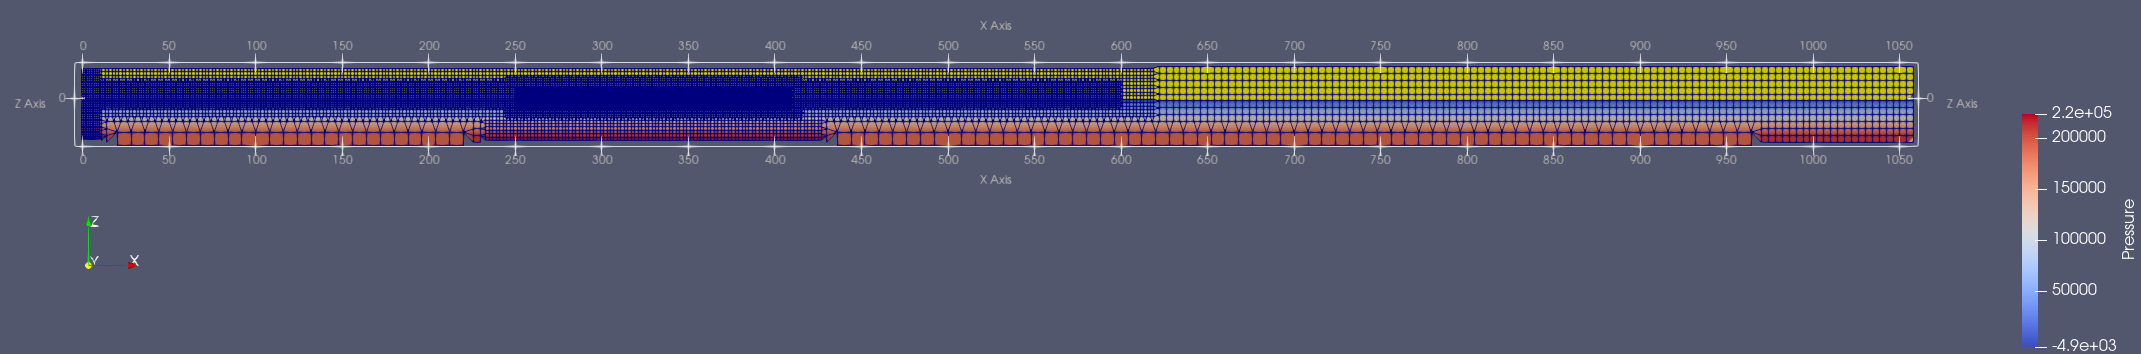
\includegraphics[width=\linewidth]{figures/Methodology/grid2.png}
    \caption{Grid used in simulations}
    \label{fig: grid used methodology}
\end{figure}

\begin{figure}[h]
    \centering
    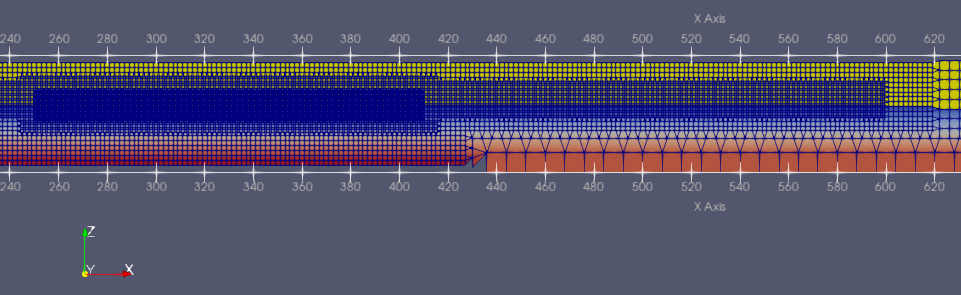
\includegraphics[width=\linewidth]{figures/Methodology/grid zoomed 2.png}
    \caption{Grid used in simulations zoomed}
    \label{fig: zoomed grid used methodology}
\end{figure}



% \section{Test of scripts}

% Breakwaters with simple geometries are used to test whether the scripting of the \acrfull{cob}, mass and radius of inertia is calculated right. These quantities can be easily determined manually for these geometries and compared to the results of the Python script. Once all these quantities match between the hand calculations and the Python scripts, it can be concluded that these quantities are calculated correctly for more complex geometries as well. The geometries from Figure \ref{tab:check breakwaters}, with its parameters given in Table \ref{tab:check breakwaters}, are used for this check.


% % Please add the following required packages to your document preamble:
% % \usepackage{booktabs}
% \begin{table}[h]
% \centering
% \begin{tabular}{@{}lllllll@{}}
% \toprule
% configuration & T [m]  & W [m]   & front\_fraction [-] & top\_fraction [-] & radius [m] & WL [m] \\ \midrule
% 1   & 10 & 100 & 0.00001            & 0.00001          & 2e7 & 2  \\
% 2   & 10 & 100 & 0.00001            & 0.00001          & 2e7 & -5 \\
% 3   & 10 & 100 & 0.99999            & 0.99999          & 2e7 & 2  \\
% 4   & 10 & 100 & 0.99999            & 0.99999          & 2e7 & -5 \\ 
% 5   & 10 & 100 & 0.50            & 0.50          & 2e7 & -8 \\ \bottomrule
% \end{tabular}
% \caption{Parameters of breakwaters}
% \label{tab:check breakwaters}
% \end{table}





% \begin{figure*}[h]
%     \centering
%     \begin{subfigure}[b]{0.475\textwidth}
%         \centering
%         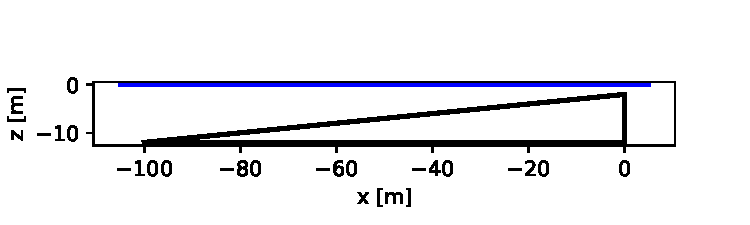
\includegraphics[width=\textwidth]{figures/ComFLOW/Breakwater Geometries/script checks/breakwater_geometry1.pdf}
%         \caption[]%
%         {{\small Configuration 1}}    
%         \label{fig: check Configuration 1}
%     \end{subfigure}
%     \hfill
%     \begin{subfigure}[b]{0.475\textwidth}  
%         \centering 
%         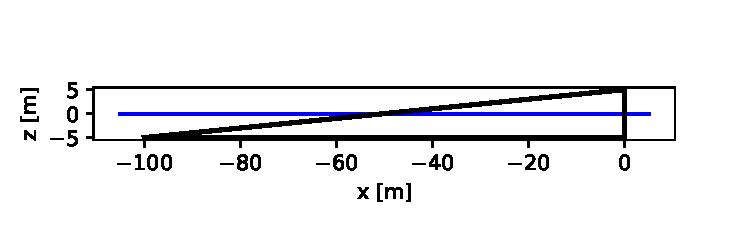
\includegraphics[width=\textwidth]{figures/ComFLOW/Breakwater Geometries/script checks/breakwater_geometry2.pdf}
%         \caption[]%
%         {{\small Configuration 2}}    
%         \label{fig: check Configuration 2}
%     \end{subfigure}
%     \vskip\baselineskip
%     \begin{subfigure}[b]{0.475\textwidth}   
%         \centering 
%         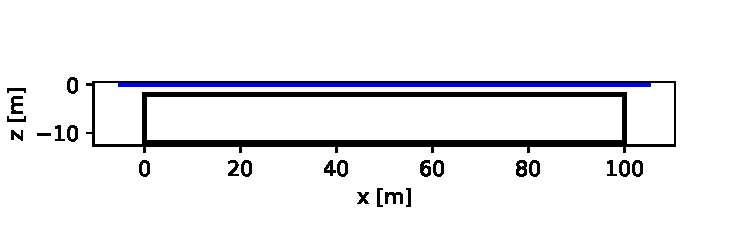
\includegraphics[width=\textwidth]{figures/ComFLOW/Breakwater Geometries/script checks/breakwater_geometry3.pdf}
%         \caption[]%
%         {{\small Configuration 3}}    
%         \label{fig: check Configuration 3}
%     \end{subfigure}
%     \hfill
%     \begin{subfigure}[b]{0.475\textwidth}   
%         \centering 
%         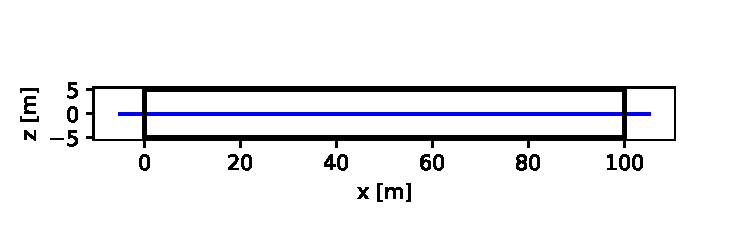
\includegraphics[width=\textwidth]{figures/ComFLOW/Breakwater Geometries/script checks/breakwater_geometry4.pdf}
%         \caption[]%
%         {{\small Configuration 4}}    
%         \label{fig: check Configuration 4}
%     \end{subfigure}
%     \hfill
%     \begin{subfigure}[b]{0.475\textwidth}   
%         \centering 
%         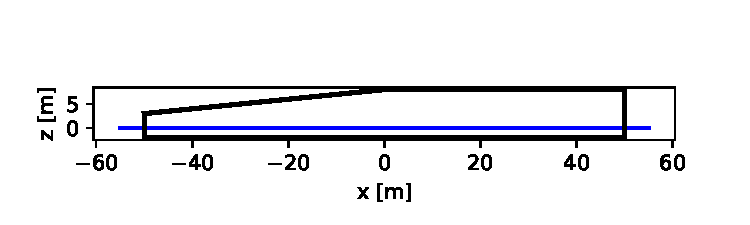
\includegraphics[width=\textwidth]{figures/ComFLOW/Breakwater Geometries/script checks/breakwater_geometry5.pdf}
%         \caption[]%
%         {{\small Configuration 5}}    
%         \label{fig: check Configuration 5}
%     \end{subfigure}
%     \caption{Breakwaters}
%     \label{fig: check Configurations}
% \end{figure*}


% The Python scripts which calculated the mass of the breakwater and the location of the acrfull{cog} for each configuration performed well according to this test. This can be seen in Table \ref{tab:check values hand cal vs P}, where all numbers complied. Except for the location of the acrshort{cog} for configurations where the beach of the breakwater is either partly or fully under water. There they were 1 to 4 cm off, which is negligible on such scales and due to numerical errors in the calculations. 


% \begin{table}[h]
% \begin{tabular}{lllllll}
% \hline
%               & \multicolumn{3}{l}{Hand calculations}                   & \multicolumn{3}{l}{Values Python scripts}               \\ \hline
% configuration & mass {[}kg{]} & x$_{CoG}$ {[} m{]} & z$_{CoG}$ {[} m{]} & mass {[}kg{]} & x$_{CoG}$ {[} m{]} & z$_{CoG}$ {[} m{]} \\ \hline
% 1 & 5.00e5 & -33.33 & -6.67 & 5.00e5 & -33.37 & -6.67 \\
% 2 & 3.75e5 & -38.89 & -7.77 & 3.75e5 & -38.86 & -7.78 \\
% 3 & 1.00e6 & 50.00  & -5.00 & 1.00e6 & 50.00  & -5.00 \\
% 4 & 5.00e5 & 50.00  & -7.50 & 5.00e5 & 50.00  & -7.50 \\
% 5 & 2.00e5 & 50.00  & -9.00 & 2.00e5 & 50.00  & -9.00 \\ \hline
% \end{tabular}
% \caption{Values of hand calculations versus values out of Python scripts}
% \label{tab:check values hand cal vs P}
% \end{table}


% Also, with these and more floaters still water tests are performed, where the breakwater were tested for 300 seconds in the water without the interference with waves to see whether the mass and acrshort{cog}  are scripted correctly. No strange behaviour was observed, the breakwaters did not move.



\section{Cost Function}
\label{sec: cost analysis methodology }
In this section the cost function is introduced which determines the total cost reduction on the system due to the presence of the breakwater. This cost function consists of three parts. In the first part, the mooring system of the floating island of the North Sea case of Space@Sea is decomposed in \ref{sec: mooring costs}. This is used to determine the cost reduction provided by the breakwater, which is discussed in Section \ref{eq: reduction mooring costs}. Finally, the construction costs of the breakwater are estimated using a cost function presented in Section \ref{sec: breakwater costs}.



%Also, the floating island will experience less motions when the right breakwater is placed, which increases the workability on the island modules and connector costs will be less. Therefore, a cost function which quantifies these effects as function of the breakwaters transmitted wave height will be introduced in Section \ref{sec: work and connector costs}.


\subsection{Mooring costs}
\label{sec: mooring costs}

% An estimation was made for the mooring costs by using the the public deliverable D1.3 from Space@Sea. In this document is referred to a document where the exact composition of the mooring costs can be found. Unfortunately, this document is confidential. Thereby, an estimation was made by the following calculation. D1.3 gave a total of \texteuro 20 M for the total mooring system of the floating island, schematized by the following picture

% -estimation mooring costs Space@Sea\\
% -Delivarable 1.3: total mooring system costs \texteuro 20 M\\
% -So, one row of breakwaters would cost roughly \texteuro 20/9 M.
% -That mean wave drift force scales linearly with the amount of euros 


In Space@Sea, extensive research is done by \citet{D3.3space@sea} on the design of the mooring system of the North Sea case, based on the wind, wave and current conditions at that location (see Section \ref{sec:intro background} for the exact location). This design of the mooring system, with its costs, is taken as a benchmark for estimating the reduction in mooring costs. First, we investigate how the mooring design was constructed in order to make an as accurate as possible cost function for the future mooring costs of what the mooring system would cost when a breakwater is present. The total costs of the mooring system was estimated by \citet{D3.3space@sea} at \texteuro 20 M. Since a 2D breakwater is studied in this thesis, everything is calculated per unit width. Therefore, this set-up is simplified to a single row of nine island modules. It is assumed that this will cost $\frac{1}{9}$ of the total mooring costs, which is approximately \texteuro 2.22 M. Dividing this by 45 (= module width) leads to \texteuro 49.382,71 per unit width of the floating island.  This design is made based on a peak mean wave drift force of 120.7 MN, which is caused by the wind, current, and waves. In the following sections, the magnitude of the contribution of each phenomenon is investigated. 


\begin{figure}[h]
    \centering
    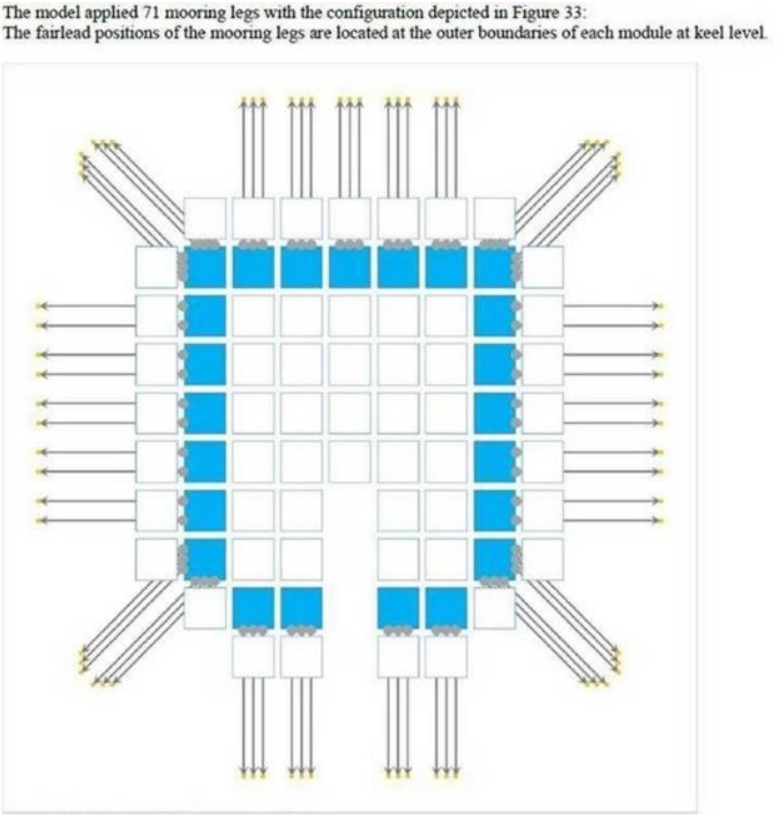
\includegraphics[width=0.5\linewidth]{figures/Costs/mooring_layout.PNG}
    \caption{Mooring layout Space@Sea. Source: \citep{S@S1.3}}
    \label{fig: mooring layout S@S}
\end{figure}



\paragraph{Wind Load}
The contributions of the wind loads are applied using the following \acrfull{OCIMF} convention \cite{D3.3space@sea}:
\begin{equation}
    F_{x,w} = \frac{1}{2} \cdot \rho_a \cdot C_{x,w} \cdot V_w^2 \cdot A_T
\end{equation}
In the design of the Space@Sea mooring system, the following parameters are used:
\begin{itemize}
    \item Air density $\rho_a$ = 1.225 $kg/m^3$
    \item Coefficient $C_{x,w}$ = 1
    \item Wind velocity $V_w$ = 29.5 $m/s$
    \item Transverse surface area above water $A_T$ = 225 $m^2$
\end{itemize}
This results in a design wind load per unit width of $F_{x,w}~\approx$ 239.86 kN. Dividing this through the width of the floater gives a wind design load of $F_{x,w}~\approx$ 5.33 kN/m

\paragraph{Current Load}
The current load used for the design of the Space@Sea mooring system is calculated according to the \acrshort{OCIMF} convention as well:
\begin{equation}
    F_{x,w} = \frac{1}{2} \cdot \rho_w \cdot C_{x,c} \cdot V_c^2 \cdot W \cdot T
\end{equation}
where the following parameters are used:
\begin{itemize}
    \item Seawater Density $\rho_w$ = 1000 $kg/m^3$
    \item Coefficient $C_{x,c}$ = 1
    \item Current velocity $V_c$ = 2.0 $m/s$
    \item Module width $W$ = 45 $m$
    \item Module depth $T$ = 6 $m$
\end{itemize}
This results in a current design load of $F_{x,c}~ = $ 540.00 kN. Per unit width this is $F_{x,c}~ = $ 12.00 kN/m\\
\\
\paragraph{Wave load}
The maximum mean wave drift force used in the design of the mooring system of the entire island (see Figure \ref{fig: mooring layout S@S}) is 120.7 MN \cite{D3.3space@sea}. Per unit width, this is 297.93 kN/m. From which 12.00 kN/m is due to the current and 5.33 kN/m is due to the wind. So, the contribution to the mean wave drift force delivered by the waves is 280.60 kN/m, which is 94 \% of the total mean wave drift force.\\
\\
This big proportion of the contribution of the waves to the maximum mean wave drift on the island emphasises the potential added value the breakwater can have, but does not mean that we can neglect the other contributions by the wind and the current. Six per cent may seem negligible, but when a breakwater succeeds in attenuating the waves substantially, these ratios will be very different. Especially since the height of the mean wave drift force on the floating island scales to the height of the waves interacting with the island squared. Therefore, the breakwater can only contribute in lowering 94\% of this force, the 6\% due to the wind and current will always stay included. This is more elaborated in the folowing section. 


\subsection{Reduction of mooring costs due to the presence of breakwater}
\label{subsec: reduction mooring costs function}
This section explains how the results of the last section are used for the cost function of the cost reduction in mooring costs, due to the presence of the breakwater. First, the cost function is symbolically shown in equations \ref{eq: new mooring island costs} to \ref{eq: reduction mooring costs}, using the relations shown in \ref{eq: relations cost function}. Then, the same cost function is clarified using text and figures.



% The rest of the section explains how the reduction of mean wave drift forces on the floating island quantifies in a reduction of mooring costs. In \cite{D3.3space@sea} is stated that the mooring system is designed for a peak mean wave drift force of 120.7 MN. To convert this to a single row of modules again, $\frac{1}{9}$th of that force will be 13.4 MN and dividing this through 45 leads to 0.30 MN of design drift force per unit with of floating island. The mean wave drift force scales to the height of the incoming wave squared. Together with the assumption that the cost of the mooring system scales linearly to the mean wave drift force acting on the island, the reduction on mooring costs is derived as follows.


\begin{equation}
\begin{array}{lll}
    H^2 & \propto \bar{F_d}\\
    \\
    \bar{F_d} & \propto \texteuro_{mooring} \\
    \\
    \texteuro_{mooring} & \propto H^2
\end{array}
\label{eq: relations cost function}
\end{equation}


% \begin{equation}
% \begin{array}{lll}
%     \text{\texteuro}_{new~mooring~island} = \text{\texteuro}_{old~mooring~island} \cdot \frac{H_{t,breakwater}}{H_{i,breakwater}}^2\\
%     \\
%     \text{\texteuro}_{mooring~breakwater} = \text{\texteuro}_{old~mooring~island} \cdot \frac{\bar{F_{d, breakwater}}}{F_{peak S@S island}}\\
%     \\
%     \text{\texteuro}_{new~total~mooring} = \text{\texteuro}_{new~mooring~island} + \text{\texteuro}_{mooring~breakwater}

% \end{array}
% \end{equation}

Leads to
\begin{equation}
    \text{\texteuro}_{new~mooring~island} =  \text{\texteuro}_{old~mooring~island} \cdot (0.06+ 0.94\cdot \frac{H_{t,breakwater}}{H_{i,breakwater}}^2)
    \label{eq: new mooring island costs}
\end{equation}
\begin{equation}
    \text{\texteuro}_{mooring~breakwater} = \text{\texteuro}_{old~mooring~island} \cdot \frac{\bar{F}_{d, breakwater}}{\bar{F_{d, old~island}}}\\
    \label{eq: mooring costs breakwater}
\end{equation}
\begin{equation}
    \text{\texteuro}_{new~total~mooring} = \text{\texteuro}_{new~mooring~island} + \text{\texteuro}_{mooring~breakwater}
    \label{eq: total mooring costs}
\end{equation}
\begin{equation}
    \texteuro_{reduction~mooring~costs}  = \texteuro_{old~mooring~island}- \texteuro_{new~total~mooring}
    \label{eq: reduction mooring costs}
\end{equation}





\begin{figure}[h]
 
    \centering
    \begin{subfigure}[b]{0.99\textwidth}
        \centering
        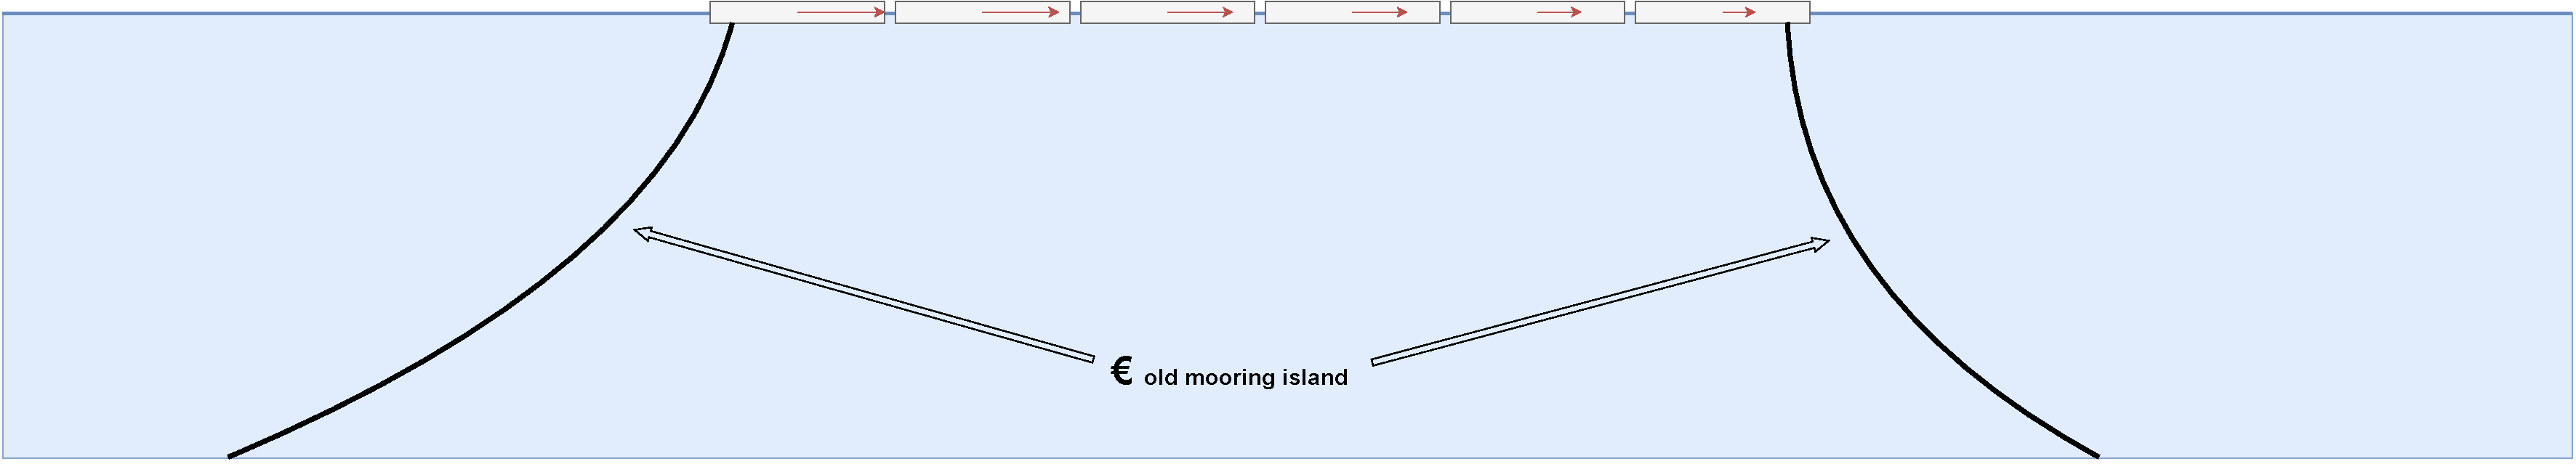
\includegraphics[width=\linewidth]{figures/Methodology/floatingisland_oldmooring.pdf} 
        \caption[]%
        {{\small Floating island without breakwater}}    
        \label{fig: old floating island cost function}
    \end{subfigure}

    \centering
    \begin{subfigure}[b]{0.99\textwidth}  
        \centering 
        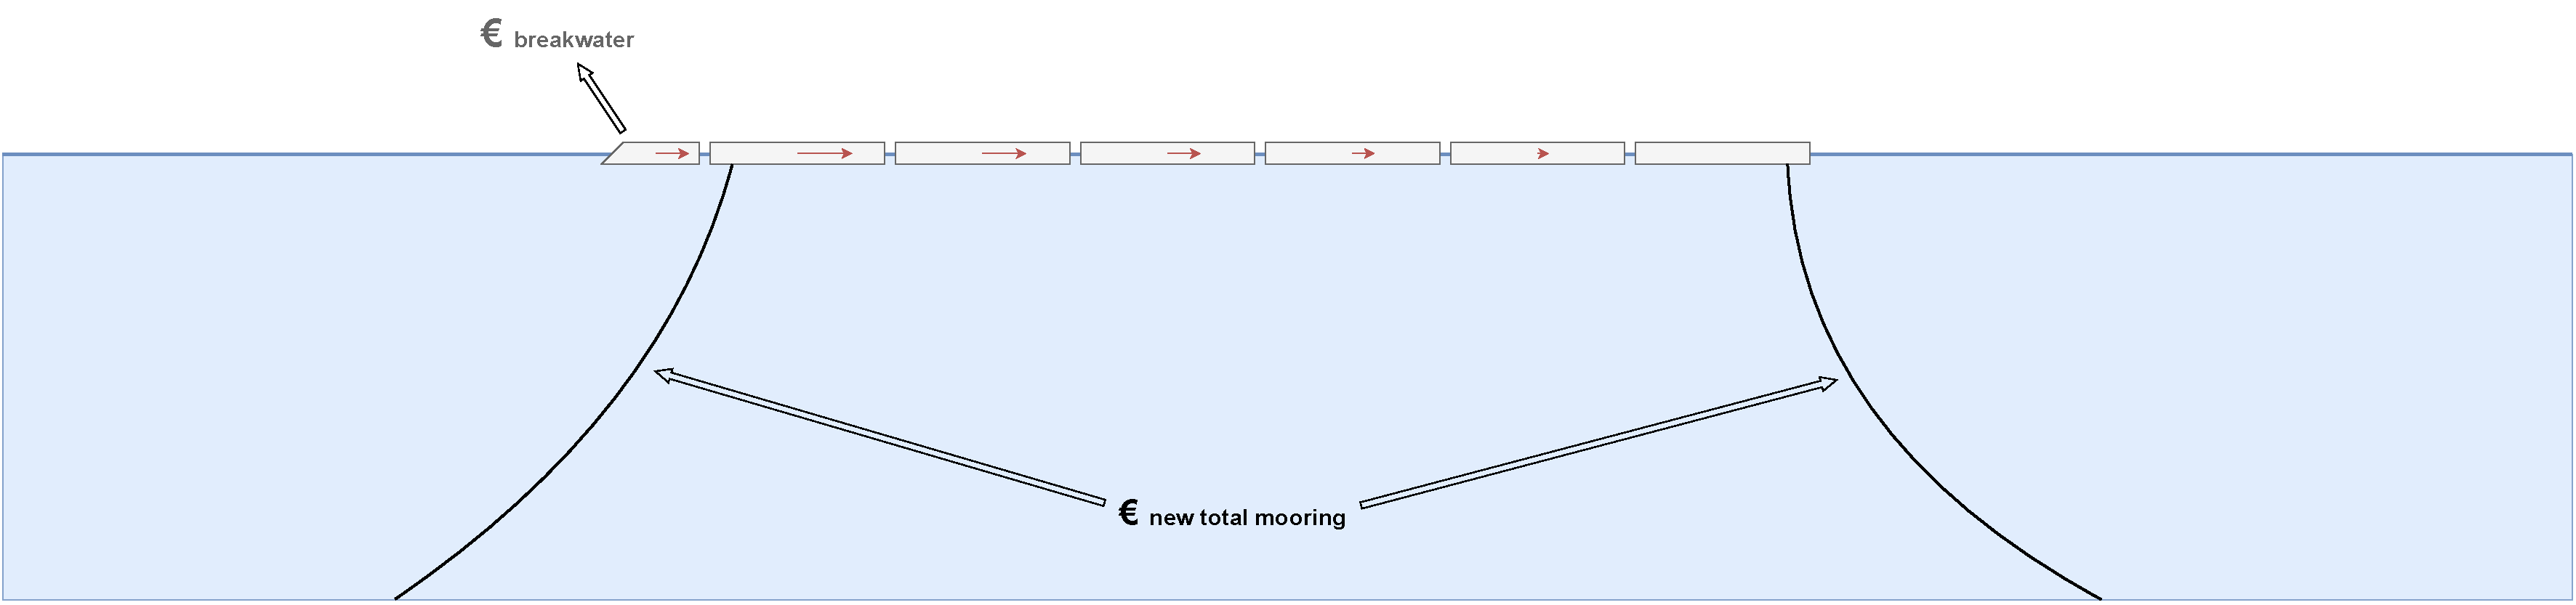
\includegraphics[width=\linewidth]{figures/Methodology/floatingisland_newmooring.pdf}
        \caption[]%
        {{\small Floating island with breakwater}}    
        \label{fig: new floating island cost function}
    \end{subfigure}



    \caption{}
    \label{fig: }
\end{figure}





The "old" floating island is the Space@Sea North Sea case, without breakwater, is schematically shown in Figure \ref{fig: old floating island cost function}. The mean wave drift force must be countered with a mooring system. The costs of this mooring system of the "old" floating island are denoted by \texteuro$_{old~mooring~island}$ and have a value of 49.382,71 \texteuro/m. 


The "new" floating island is the same system, but with a breakwater connected to its wave-ward side. This system is schematically shown in Figure \ref{fig: new floating island cost function}. The total mooring costs of this "new" floating island are denoted by \texteuro$_{new~total~mooring}$, which is constructed by the mooring costs of the breakwater and the new mooring costs of the island. The new mooring costs for the island are denoted by \texteuro$_{new~mooring~island}$ and will be lower than \texteuro$_{old~mooring~island}$, because the breakwater attenuates the wave energy. The transmitted wave height (wave height behind the breakwater) still causes the floating island at its lee-side to have a mean wave drift force. Therefore, the ratio between the transmitted wave height and the incident wave height is used in the calculation of \texteuro$_{new~mooring~island}$ in Equation \ref{eq: new mooring island costs}.  As can be seen in this equation, the transmission coefficient ($H_t/H_i$) has only an influence on 94\% of the new mooring costs. In other words, when 100\% of the wave is attenuated by the breakwater ($H_t/H_i$ = 0), there are no drift forces due to the waves, but the current and wind can still put a load on the mooring lines and 6\% of the old mooring costs will still be present.\\
The breakwater itself also experiences a mean drift force of the waves, which contributes to the total costs of the mooring system. This contribution is denoted by \texteuro$_{mooring~breakwater}$ and is calculated by the ratio of its mean wave drift force $\bar{F}_{d, breakwater}$ and the maximum mean wave drift force used in the design of the "old" mooring system: F$_{d, old~island}$, which is 0.30 MN/m (120.7 MN computed to per unit width). \\
Finally, the total reduction in mooring costs due to the presence of the breakwater, denoted with \texteuro$_{reduction~mooring~costs} $ is the difference between the costs of the "old" mooring system and the "new" system (equation \ref{eq: reduction mooring costs}).



% which is computed via the ratio between the transmitted wave height and the incident wave height



% The breakwater attenuates the wave energy and thereby reduces the mean wave drift force experienced by the island. 


% All quantities are per unit width. In the formula \ref{eq: new mooring island costs}, the design mooring costs of \texteuro 49.382,71 is used for $\text{\texteuro}_{old~mooring~island}$, and the ratio between the transmitted wave height and the incident wave height is used with the calculation of $\text{\texteuro}_{new~mooring~island}$, which is the new height off the mooring costs of the floating island due to the wave attenuation of the breakwater. The transmission coefficient ($H_t/H_i$) has only an influence on 94\% of the new mooring costs. In other words, when 100\% of the wave is attenuated by the breakwater ($H_t/H_i$ = 0), no drift forces are present due to the waves, but the current and wind can still give a load on the mooring lines and 6\% of the old mooring costs will still be present.\\
% Formula \ref{eq: mooring costs breakwater} defines the costs of the mooring system of the breakwater itself, using again the design costs of the floating island of Space@Sea times the ratio of the mean wave drift force on the breakwater and the mean wave drift force where the design mean wave drift force of the Space@Sea island. Note that this quantity can be negative when a negative mean wave drift force on the breakwater is experienced.\\



% The outcome of the two latter formulas leads to the total costs of the mooring system: $\text{\texteuro}_{new~total~mooring}$ in formula \ref{eq: total mooring costs} and this is used to calculate the eventual reduction in mooring costs due to the presence of the breakwater $\texteuro_{reduction~mooring~costs}$ in \ref{eq: reduction mooring costs}.








\subsection{Breakwater costs}
\label{sec: breakwater costs}


For the costs of the breakwater, it is assumed that the construction is made of steel and concrete. This material is relatively inexpensive and makes a good combination because concrete is resistant to compression and steel to tension, while they have roughly the same thermal expansion coefficient. In Deliverable 1.2 of the Space@Sea project (\cite{Adam2017D1.2S@S}), a business case is made for an energy hub that aims to provide accommodation and work space for offshore workers. Comprehensive research is done on what the costs would be of such floating structures. Here, it is estimated that the steel and concrete carcass of the structure would have a mass of 9300 ton and would cost \texteuro 9.611.077. From this 9300 ton, 5407 ton (58\%) would be steel and 3893 ton (42\%) concrete. The price of concrete is roughly 775 \texteuro/ton and the price of steel varies from 2000 \texteuro/ton to 4000 \texteuro/ton, depending on the labour needed to manufacture the construction. These prices and mass ratios are used to estimate the \acrshort{capex} costs of the breakwater. So the height of the steel price is different for each breakwater. A box-type structure can be made for 2000 \texteuro/ton and a skew floating beach can be made for 4000 \texteuro/ton. This variation is made into a function the following way; the rectangular parts of the breakwater are made for 2000 \texteuro/ton and the variable part varies between 2000 and 4000 \texteuro/ton (red part in Figure \ref{fig: steel price breakwater}), depending on the angle $\alpha$ with the following formula:
\begin{equation}
    for ~ 0\textdegree ~\alpha<45 \textdegree~:~ \texteuro_{steel} = 4 - \frac{2}{45} \cdot alpha
\end{equation}
\begin{equation}
        for ~ 45\textdegree~<\alpha<90\textdegree ~:~\texteuro_{steel} =\frac{2}{45} \cdot alpha
\end{equation}
\begin{figure}
    \centering
    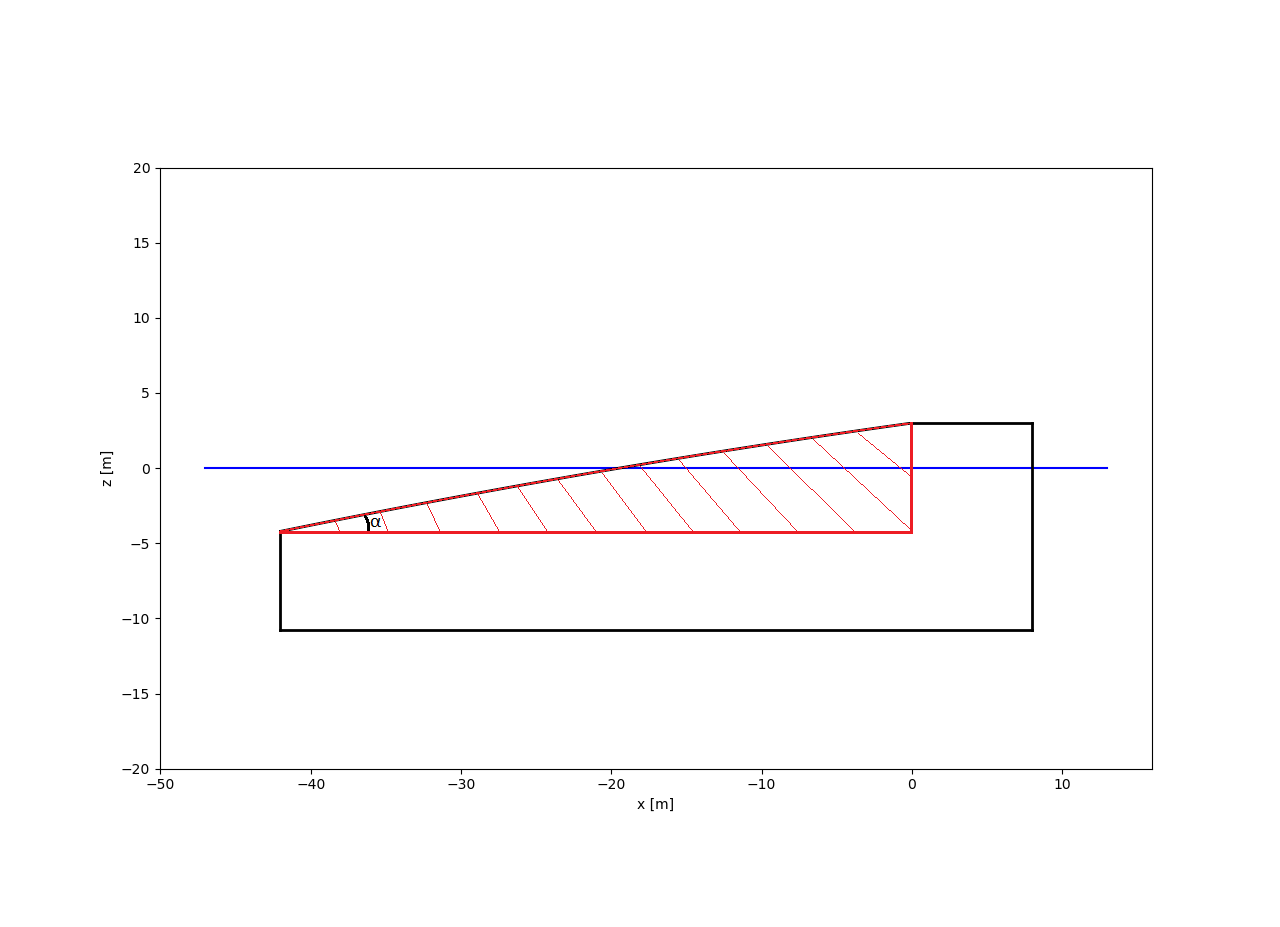
\includegraphics[width=0.5\linewidth]{figures/Costs/breakwater_1.png}
    \caption{Part where steel price is variable}
    \label{fig: steel price breakwater}
\end{figure}
In this way, the price reaches its maximum (4000 \texteuro/ton) when a very skew slope is desired and its minimum (2000 \texteuro/ton) when $\alpha=45 \textdegree$. \\
\\
Now the prices for all parts of the breakwater are known. The only thing missing is the total price of the structure. Therefore, the energy hub of the Space@Sea project is again taken as a benchmark. The steel and concrete carcass of this hub will be approximately \texteuro 9.611.077 and have dimensions of: WxBxH = 45m x 45m x 10 m. Per unit width, the price is approximately 213.580 \texteuro/m. Dividing this by the circumference in the xz-plane (45$\cdot$10=450 m$^2$) results in approximately 475 \texteuro/m$^3$, which is the price of the steel and concrete carcass of the energy hub per unit width per unit circumference. Multiplying this number by the circumference of the breakwater almost gives the construction price of the breakwater. The only thing left to do is multiply the result by a fraction so that the steel used on the beach slope is made for the variable steel price and the steel used on the rest of the breakwater for \texteuro 2000 euro/ton. The way this price is calculated in Python is shown in the function '\textit{geometry\_costs\_function2}' in Appendix \ref{app: scripts for post-processing}.\\
\\
Of course, the market price of concrete can also vary in time, but the amount of labour put into the manufacturing of the concrete is hardly affected by the shape of the breakwaters. It is poured in fluidly after the framework is created and takes on the proper shape by itself. Thus, the price of concrete is assumed to be constant with a price of 775 \texteuro/ton for the breakwaters. \\

